% file: CUDACFD_writeup01.tex
% CUDA + CFD (Computational Fluid Dynamics)
% 
% github        : ernestyalumni
% gmail         : ernestyalumni 
% linkedin      : ernestyalumni 
% wordpress.com : ernestyalumni
%
% This code is open-source, governed by the Creative Common license.  Use of this code is governed by the Caltech Honor Code: ``No member of the Caltech community shall take unfair advantage of any other member of the Caltech community.'' 

\documentclass[10pt]{amsart}
\pdfoutput=1
\usepackage{mathtools,amssymb,lipsum,caption}

\usepackage{graphicx}
\usepackage{hyperref}
\usepackage[utf8]{inputenc}
\usepackage{listings}
\usepackage[table]{xcolor}
\usepackage{pdfpages}
\usepackage{tikz}
\usetikzlibrary{matrix,arrows}

\usepackage{breqn} % for dmath


\usepackage{cancel} % for Feynman slash notation

\hypersetup{colorlinks=true,citecolor=[rgb]{0,0.4,0}}


%\oddsidemargin=15pt
%\evensidemargin=5pt
%\hoffset-45pt
%\voffset-55pt
%\topmargin=-4pt
%\headsep=5pt
%\textwidth=1120pt
%\textheight=595pt
%\paperwidth=1200pt
%\paperheight=700pt
%\footskip=40pt








\newtheorem{theorem}{Theorem}
\newtheorem{corollary}{Corollary}
%\newtheorem*{main}{Main Theorem}
\newtheorem{lemma}{Lemma}
\newtheorem{proposition}{Proposition}

\newtheorem{definition}{Definition}
\newtheorem{remark}{Remark}

\newenvironment{claim}[1]{\par\noindent\underline{Claim:}\space#1}{}
\newenvironment{claimproof}[1]{\par\noindent\underline{Proof:}\space#1}{\hfill $\blacksquare$}

%This defines a new command \questionhead which takes one argument and
%prints out Question #. with some space.
\newcommand{\questionhead}[1]
  {\bigskip\bigskip
   \noindent{\small\bf Question #1.}
   \bigskip}

\newcommand{\problemhead}[1]
  {
   \noindent{\small\bf Problem #1.}
   }

\newcommand{\exercisehead}[1]
  { \smallskip
   \noindent{\small\bf Exercise #1.}
  }

\newcommand{\solutionhead}[1]
  {
   \noindent{\small\bf Solution #1.}
   }


\title{Using CUDA C/C++ for Computational Fluid Dynamics (CFD)}
\author{Ernest Yeung \href{mailto:ernestyalumni@gmail.com}{ernestyalumni@gmail.com}}
\date{9 ao\^{u}t 2016}
\keywords{CUDA C/C++, Computational Fluid Dynamics, Euler equations, Compressible fluid dynamics, gas dynamics}

\begin{document}

\definecolor{darkgreen}{rgb}{0,0.4,0}
\lstset{language=Python,
 frame=bottomline,
 basicstyle=\scriptsize,
 identifierstyle=\color{blue},
 keywordstyle=\bfseries,
 commentstyle=\color{darkgreen},
 stringstyle=\color{red},
 }
%\lstlistoflistings

\maketitle

\tableofcontents

%\begin{multicols*}{2}

\begin{abstract}
  This is a writeup for using CUDA C/C++ for parallel programming on the GPU (Graphics Processing Unit), or GPGPU (General Programming on a GPU), for Computational Fluid Dynamics (CFD).  I briefly describe an implementation of the so-called ``Upwind'' scheme for finite volume methods for convection in 1-dimensional and 3-dimensional case, implemented to run in parallel on the GPU.

  Then I describe the implementation of finite difference methods.  I've shown how the coefficients for the so-called forward and backward difference operators, the central difference operators can be obtained for any desired order.  I implement these coefficients on the constant memory of the GPU (CUDA C/C++); their initialization and the subsequent directional derivatives are implemented as C++ classes on the device GPU.  I use these finite difference methods to compute the heat equation in 2-dimensions and 3-dimensions.  I also use them to compute the convection (according to mass conservation) in 1-dimensions and 3-dimensions of a Gaussian-distributed ``ball'' of mass.  I will also describe my attempt at using these methods to compute the Euler equation (Navier-Stokes equations for an inviscid (i.e. nonviscous) flow, motivated by high-Reynolds number gas flow from the combustion chamber out to the nozzle in rockets) in 3-dimensions.  
\end{abstract}

\section{``Upwind'' scheme for finite volume methods}

Consider the so-called ``upwind method.''  Consider the 1-dimensional case.

Let $C_i^1 \equiv $ $i$th cell of dimension 1, for $i = 0, \dots , N-1$.  So there are $N$ total cells.

Cells are centered at $x_{2i+1} = l \frac{ (2i+1)}{2} = l(i + \frac{1}{2})$.  $l$ is the 1-dimensional size or length of a single cell.  Notice that in this case, I am assuming a uniform grid.  Note that this can be easily generalized to a grid with different cell sizes for each cell.  

For the $i$th cell, which is a 1-(cubic) simplex, a line segment, $C_i^1$, it has 2 $0$-(cubic) simplices (faces), which in this 1-dimensional case, it's 2 isolated points: $\partial C_i^1 = \lbrace C^0_{i \pm 1} \rbrace$.

The centers of these faces, i.e. the position of these 2 points, at the ends of the line segment, are
\[
x_{C^0_{i \pm 1} } = l \left( \frac{2i  +1 \pm 1 }{2} \right) = l ( i + \frac{1}{2} \pm \frac{1}{2} ) = \lbrace li, l(i+1) \rbrace
\]

I will take the mass conservation equation, in its integral form, as an example here, but this example can be easily generalized to the convection of any other conserved quantity.  Define the average mass density $\overline{\rho}_i$:
\begin{equation}
  \overline{\rho}_i := \frac{1}{l} \int_{C_i^1} \rho \text{vol}^1
\end{equation}
For the mass conservation equation (in integral form),
\begin{equation}\label{Eq:massconsvdiscretize}
\int_V  \frac{ \partial \rho}{ \partial t} = - \int_{\partial V} i_{\mathbf{u}}\rho \text{vol}^1
  \end{equation}
where the integral is taken over the volume $V$, and over its boundary $\partial V$ (which is the surface of $V$).

For the left-hand side (LHS) of Eq. \ref{Eq:massconsvdiscretize}, rewrite it in terms of $\overline{\rho}_i$,
\[
\begin{gathered}
  \int_{C_i^1} \frac{  \partial \rho}{ \partial t}(t,x) \text{vol}^1 \approx \int_{C_i^1} \frac{ \rho(t+\Delta t, x) - \rho(t,x) }{ \Delta t} \text{vol}^1 = \\
  = \frac{1}{ \Delta t} \left[ \int_{C_i^1} \rho(t+\Delta t,x) \text{vol}^1 - \int_{C_i^1} \rho(t,x) \text{vol}^1 \right] = \\
  = \frac{l}{\Delta t} \left[ \overline{\rho}_i(t+\Delta t) - \overline{\rho}_i(t) \right]
  \end{gathered}
\]

Considering the mass flux through the ``surface'' or through the endpoints of the line segment, that is a cell in the 1-dimensional case,
\[
\int_{\partial C_i^1} i_{\mathbf{u}} \rho \text{vol}^1 = \int_{ \partial C_i^1} \rho u^i dS_i
\]
then the so-called ``upwind'' scheme is this:
\[
\begin{gathered}
  \int_{C^0_{i+1}} \rho u^i dS_i = u^x(x_{C^0_{i+1}}) \int_{C^0_{i+1} } \rho dS_x = \begin{cases} 
    \overline{\rho}_iu^x(x_{C^0_{i+1}} ) & \text{ if } u^x(x_{C^0_{i+1}}) > 0 \\
    \overline{\rho}_{i+1}u^x(x_{C^0_{i+1}} ) & \text{ if } u^x(x_{C^0_{i+1}}) < 0
    \end{cases} \\
  \int_{C^0_{i-1}} \rho u^i dS_i = -u^x(x_{C^0_{i-1}}) \int_{C^0_{i-1} } \rho dS_x = \begin{cases} 
    -\overline{\rho}_{i-1}u^x(x_{C^0_{i-1}} ) & \text{ if } u^x(x_{C^0_{i-1}}) > 0 \\
    -\overline{\rho}_{i}u^x(x_{C^0_{i-1}} ) & \text{ if } u^x(x_{C^0_{i-1}}) < 0
    \end{cases} 
\end{gathered}
\]


For the 3-dimensional case, I refer back to my notes on \href{https://github.com/ernestyalumni/CompPhys/blob/master/LaTeXandpdfs/CompPhys.pdf}{Computational Physics} in the 3-dim. ``Upwind'' subsection. 


For a rectangular prism (cubic),

for cell $C^3_{ijk}$, $i=0 \dots N_x-1$, $j=0 \dots N_y-1$ , $k=0 \dots N_z-1$, $N_x\cdot N_y \cdot N_z$ total cells.

Cells centered at
\[
(x_{2i+1}, y_{2j+1}, z_{2j+1}) = (l^x \frac{ (2i+1)}{2} , l^y \frac{(2j+1)}{2}, l^z \frac{(2k+1)}{2} ) = \left( \sum_{l=0}^{i-1} l_l^x + \frac{l_i^x}{2} , \sum_{l=0}^{j-1}l_l^y + \frac{l_j^y}{2}, \sum_{l=0}^{k-1}l_l^z + \frac{l_k^y}{2}  \right)
\]
For the 3-(cubic) simplex, $C^3_{ijk}$, it has 6 2-(cubic) simplices (faces).  So for $C_{ijk}^3$, consider $\lbrace C^2_{i\pm 1, jk}, C^2_{ij\pm 1,k}, C^2_{ijk\pm 1}\rbrace$.

The center of these faces, such as for $C^2_{i\pm 1, jk}$, $x_{ C^2_{i\pm 1, jk} }$, for instance,
\[
\begin{aligned}
  x_{C^2_{i\pm 1,jk}} = (x_{2i+1\pm 1},y_{2j+1},z_{2k+1}) = (l^x\left( \frac{2i+1\pm 1}{2}\right) , l^y\frac{(2j+1)}{2},  l^z\frac{(2j+1)}{2} ) = \\
  = \left( \sum_{l=0}^{ \frac{2i - 1 \pm 1 }{2} } l_l^x, \sum_{l=0}^{j-1} l_l^y + \frac{l_j^y}{2}, \sum_{l=0}^{l-1} l_l^z + \frac{l_k^z}{2} \right) 
  \end{aligned}
\]

We want the flux.  So for
\[
\overline{\rho}_{ijk} := \frac{1}{l_i^x l_j^yl^z_k} \int_{C^3_{ijk}} \rho \text{vol}^3
\]
then the flux through 2-(cubic) simplices (faces), $\int \rho i_{\mathbf{u}}\text{vol}^3$,
\[
\begin{aligned}
 &  \int_{C^2_{i+1,jk}} \rho i_{\mathbf{u}} \text{vol}^3 = \begin{cases} l_j^yl_k^z \overline{\rho}_{ijk} u^x(x_{C^2_{i+1, jk} } ) & \text{ if } u^x(x_{C^2_{i+1,jk} }) > 0 \\ 
 l_j^y l^z_k \overline{\rho}_{i+1,jk} u^x(x_{C^2_{i+1, jk} } ) & \text{ if } u^x(x_{C^2_{i+1,jk} }) < 0 \end{cases} \\
\end{aligned}
\]
\[
\begin{gathered}
  \int_{C^2_{i-1,jk}} \rho i_{\mathbf{u}} \text{vol}^3 = \int_{C^2_{i-1,jk}} \rho u^i dS_i = \int_{C^2_{i-1,jk}} \rho u^i \frac{ \sqrt{g}}{ (3-1)!} \epsilon_{ii_2i_3} dx^{i_2} \wedge dx^{i_3} = -u^x(x_{C^2_{i-1,jk}}) \int_{C^2_{i-1,jk} } \rho dy dz = \\
  = \begin{cases}
    -l_j^y l^z_k \overline{\rho}_{i-1,jk} u^x(x_{C^2_{i-1,jk}}) & \text{ if } u^x(x_{C^2_{i-1,jk}}) > 0 \\
        -l_j^y l^z_k \overline{\rho}_{i,jk} u^x(x_{C^2_{i-1,jk}}) & \text{ if } u^x(x_{C^2_{i-1,jk}}) < 0 
    \end{cases}
\end{gathered}
\]

and so on.

\section{Finite Difference}

Much has already been said and taught about finite difference methods, namely the central difference approximation, and the forward difference operator and backward difference operators, where one uses values on grid points adjacent to the grid point of interest, where one wants to compute an approximation to the derivative of a function, of order $d$.  I will focus on the case of order $d=1,2$.  I will use the partial derivative notation even in the 1-dimensional case because we will ultimately apply the finite difference method to directional derivatives.  Also, here, I will only talk about the central difference approximation, although in the jupyter notebook I wrote up, I've provided Python code to compute out the forward and backward difference coefficients up to any order of accuracy $p$ (cf. \href{https://nbviewer.jupyter.org/github/ernestyalumni/CompPhys/blob/master/finitediff.ipynb}{finitediff.ipynb}).

For $d=1$, i.e. a derivative of first order of a function $f$ (for simplicity, suppose $f\in C^{\infty}(\mathbb{R})$, i.e. $f$ is a continuous differentiable function and so its Taylor series exists), then the finite difference method is a scheme to approximate $\frac{ \partial f}{ \partial x}$, at $x$ with the value of $f$ for points adjacent to $x$.  The process of using these adjacent values is what's called ``stencil.''  For instance, make the caveat that we can make this approximation:
\begin{equation}
 \frac{ \partial f}{ \partial x} \approx \sum_{\nu = 1}^N C_{\nu}(f(x+\nu h) - f(x-\nu h)) \left( \frac{1}{h} \right)
\end{equation}
for $h$ small enough and $N$ being the ``size'' of the stencil we'd like to use.

If we take the Taylor series expansion in the above equation for $f(x \pm \nu h)$,
\[
f(x\pm \nu h) = \sum_{j=0}^p \frac{ f^{(j)}(x) }{ j!} (\pm \nu h)^j + \mathcal{O}(h^{p+1})
\]
and plug this into the equation, we obtain a system of linear equations to solve in order to obtain $C_{\nu}$ (again this is all done explicitly in \href{https://nbviewer.jupyter.org/github/ernestyalumni/CompPhys/blob/master/finitediff.ipynb}{finitediff.ipynb}):
\[
\begin{gathered}
  \sum_{\nu = 1}^N 2C_{\nu} \nu  = 1 \\ 
 \sum_{\nu = 1}^N C_{\nu} \frac{ \nu^{2j' + 1 } }{ (2j'+1)! } =0
  \end{gathered}
\]

The jupyter notebook \href{https://nbviewer.jupyter.org/github/ernestyalumni/CompPhys/blob/master/finitediff.ipynb}{finitediff.ipynb} has Python code that'll compute these coefficients $C_{\nu}$ to any order of accuracy $p$ desired for the Taylor series expansion.  What I've found is that for $d=1$,
\[
\begin{gathered}
  C_1 = \frac{1}{2} \qquad \, \text{ for } p = 1  \text{ (obviously) }
\end{gathered}
\]
\[
\begin{gathered}
  C_1 = \frac{2}{3}, \, C_2 = \frac{-1}{12} \qquad \, \text{ for } p = 3  
\end{gathered}
\]
\[
\begin{gathered}
  C_1 = \frac{3}{4}, \, C_2 = \frac{-3}{20}, \, C_3 = \frac{1}{60} \qquad \, \text{ for } p = 5  
\end{gathered}
\]
\[
\begin{gathered}
  C_1 = \frac{4}{5}, \, C_2 = \frac{-1}{5}, \, C_3 = \frac{4}{105}, \, C_4 = \frac{-1}{280} \qquad \, \text{ for } p = 7  
\end{gathered}
\]
I want to emphasize that for a stencil of size $N=2,3$ or even $N=4$, the error is described by $\mathcal{O(h^p)}$ is of order $p=3,5,7$, respectively.  So for $h$ small, we can obtain accurate estimates of the first order derivative $\frac{ \partial f}{ \partial x}$.

Likewise, for $d=2$, the coefficients $C_{\nu}$ to estimate the double derivative $\frac{ \partial^2 f}{ \partial x^2}$ can be easily obtained to any desired order of accuracy, $p$.  This double derivative estimate will be useful in computing numerically the Laplacian $\Delta$ for the heat equation.  Again, see \href{https://nbviewer.jupyter.org/github/ernestyalumni/CompPhys/blob/master/finitediff.ipynb}{finitediff.ipynb} for the Python code that implements this and determines the coefficients.  What's useful that I've used for my implementations in CUDA C/C++ are the following: for $d=2$, the coefficients $C_{\nu}$ used in the central difference operator to estimate $\frac{\partial^2 f}{ \partial x^2}$, i.e.
\[
\frac{ \partial^2 f}{ \partial x^2} = \sum_{\nu = 1}^N C_{\nu} (f(x+\nu h) + f(x-\nu h) - 2f(x)) \left( \frac{1}{h^2} \right)
\]
are, for $p=1$,
\[
C_{1} = 1
\]
for $\mathcal{O}(h)$, for $p=2$,
\[
C_1 = \frac{4}{3}, \, C_2 = \frac{-1}{12}
\]
for $\mathcal{O}(h^4)$, for $p=3$
\[
C_1 = \frac{3}{2}, \, C_2 = \frac{-3}{20}, \, C_3 = \frac{1}{90}
\]
for $\mathcal{O}(h^6)$
\[
C_1 = \frac{8}{5}, \, C_2 = \frac{-1}{5}, \, C_3 = \frac{8}{315}, \, C_4 = \frac{-1}{560}
\]
for $\mathcal{O}(h^8)$.  

\subsection{ $\text{div}$, $\text{grad}$, Laplacian $\Delta$ in finite difference }

Since we can compute directional derivatives with finite difference methods, we can easily construct $\text{div}$, $\text{grad}$, and Laplacian $\Delta $ operators.

Recall what $\text{div}$, $\text{grad}$, $\Delta$ are:
\[
\begin{aligned}
  & \text{div} : \mathfrak{X}(N) \to \mathbb{R} \\ 
  & \text{div}\mathbf{u} = \frac{1}{\sqrt{g}} \frac{ \partial }{ \partial x^i} (u^i \sqrt{g}) \xrightarrow{ g = 1} \frac{ \partial u^i}{ \partial x^i} = \frac{ \partial u^x}{ \partial x} +  \frac{ \partial u^y}{ \partial y} +  \frac{ \partial u^z}{ \partial z}
  \end{aligned}
\]
\[
\begin{aligned}
  & \text{grad}: C^{\infty}(N) \to TN \\ 
  & \text{grad}f = \frac{ \partial f}{ \partial x^j} g^{ji} \frac{ \partial }{ \partial x^i} \xrightarrow{g=1} \frac{ \partial f}{ \partial x^i} \frac{ \partial }{ \partial x^i} = \frac{ \partial f}{ \partial x} \mathbf{e}_x + \frac{ \partial f}{ \partial y} \mathbf{e}_y + \frac{ \partial f}{ \partial z} \mathbf{e}_z
  \end{aligned}
\]
\[
\begin{aligned}
  & \Delta : C^{\infty}(N) \to \mathbb{R} \\ 
  & \Delta T = \text{div}(\text{grad} T) \xrightarrow{ g= 1} \frac{ \partial^2 T}{ \partial (x^i)^2 } = \frac{ \partial^2 T}{ \partial x^2 } + \frac{ \partial^2 T}{ \partial y^2 } + \frac{ \partial^2 T}{ \partial z^2 } 
  \end{aligned}
\]

Thus, given a stencil, which would be a C/C++ array of floats or \verb|float3|s (for a $C^{\infty}$ function or vector field, respectively), then $\text{div}$, $\text{grad}$ and $\Delta $ can be calculated at a grid point by the device GPU.  This is implemented in the \verb|commonlib\| directory in the classes in \verb|finitediff.cu|, \verb|finitediff.h|.

It should also be noted that in the implementation in CUDA C/C++, the coefficients $C_{\nu}$ for finite difference ``sit on'' or are loaded in the constant memory of the device GPU, a read-only cache.  Constant memory in CUDA C/C++ works well in storing physical parameters that are frequently being called upon or used.  Empirically, I've found that it saves about low to mid single-digit percentage of the total kernel run time over ``hard-coding'' the values locally on every kernel run.  





\section{Spacetime $M$, Spatial manifold $N$ for space, discretization (functor) to the grid}
%\section{Spatial (smooth) $N$ manifold $\Longleftrightarrow$ Grid }
Physics occurs on a spacetime manifold $M$, and from Newton's laws, there is an implied foliation of the spacetime manifold into $M=\mathbb{R}\times N$, with time $t\in \mathbb{R}$ parametrizing the \emph{spatial} manifold $N$ (this is the case even in some relativistic models, e.g. ADM model).  $N$ is usually $\mathbb{R}^3$, the 3-dimensional Euclidean space.  

The desire for numerical computational necessitates the need to ``discretize'' $\mathbb{R}^3$ into grid points, $(\mathbb{Z}^+)^3$.  For example, I considered a cube, a submanifold in $\mathbb{R}^3$ with boundary, of dimensions (i.e. length, width, depth) $l_x,l_y,l_z$.  That is to represented by the computer as a set of grid points say $\lbrace 0, 1 \dots L_x \rbrace \times \lbrace 0, 1 \dots L_y \rbrace \times \lbrace 0, 1 \dots L_z \rbrace \subset (\mathbb{Z}^+)^3$ which I'll denote, for lack of better notation, as $(L_x,L_y,L_z)$.  

\[
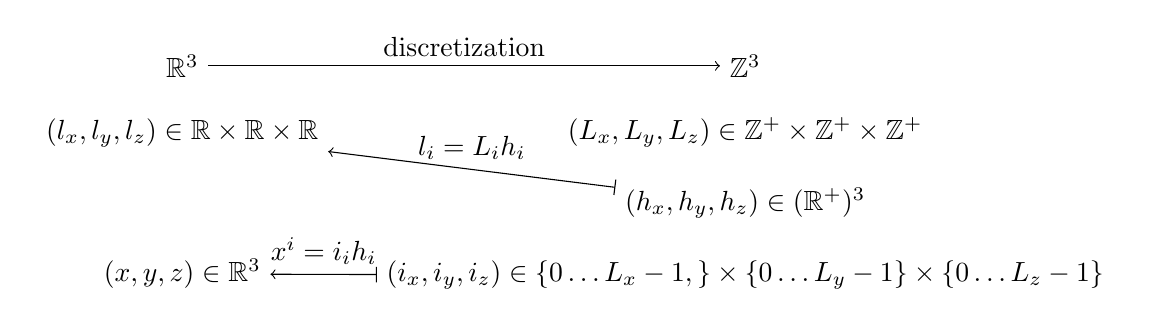
\begin{tikzpicture}
  \matrix (m) [matrix of math nodes, row sep=0.8em, column sep=1.8em, minimum width=0.6em] 
  {
    \mathbb{R}^3 & \mathbb{Z}^3 \\
    (l_x,l_y,l_z) \in \mathbb{R}\times \mathbb{R} \times \mathbb{R} & (L_x, L_y,L_z) \in \mathbb{Z}^+ \times \mathbb{Z}^+ \times \mathbb{Z}^+ \\
    & (h_x,h_y,h_z) \in (\mathbb{R}^+)^3 \\
    (x,y,z) \in \mathbb{R}^3 & (i_x,i_y,i_z) \in \lbrace 0 \dots L_x-1, \rbrace \times \lbrace 0 \dots L_y-1 \rbrace \times \lbrace 0 \dots L_z - 1\rbrace \\
    };
  \path[->]
  (m-1-1) edge node [above] {\text{discretization}} (m-1-2)
  ;
  \path[|->]
  (m-3-2) edge node [above] {$l_i = L_i h_i $} (m-2-1)
  (m-4-2) edge node [above] {$x^i = i_i h_i$ } (m-4-1)
  ;
\end{tikzpicture} 
\]

There is a \emph{flatten} functor that is necessitated by either the contiguous architecture of memory addresses on memory of the device GPU or by software constraints (CUDA C/C++ 7.5 Toolkit doesn't take multidimensional arrays).

{\small
\[
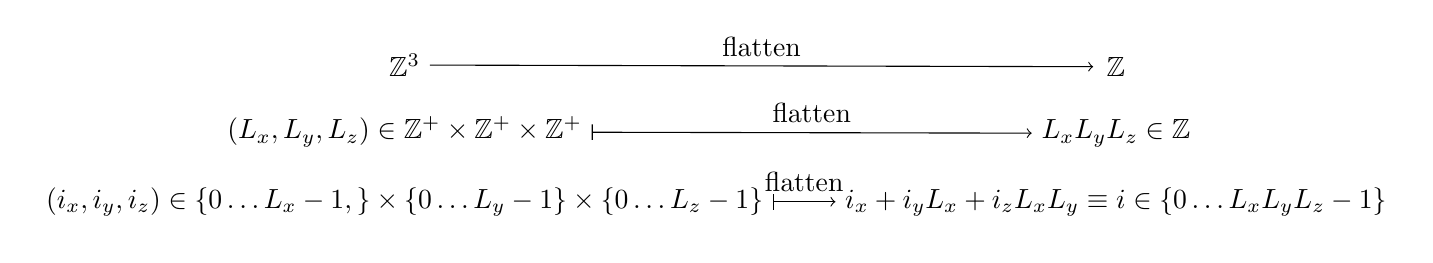
\begin{tikzpicture}
  \matrix (m) [matrix of math nodes, row sep=0.8em, column sep=2.3em, minimum width=1.6em] 
  {
     \mathbb{Z}^3 & \mathbb{Z} \\
     (L_x, L_y,L_z) \in \mathbb{Z}^+ \times \mathbb{Z}^+ \times \mathbb{Z}^+ & L_x L_y L_z \in \mathbb{Z} \\
 (i_x,i_y,i_z) \in \lbrace 0 \dots L_x-1, \rbrace \times \lbrace 0 \dots L_y-1 \rbrace \times \lbrace 0 \dots L_z - 1\rbrace & i_x + i_y L_x +i_z L_x L_y \equiv i \in \lbrace 0 \dots L_x L_y L_z-1 \rbrace \\
    };
  \path[->]
  (m-1-1) edge node [above] {\text{flatten}} (m-1-2)
  ;
  \path[|->]
  (m-2-1) edge node [above] { \text{flatten} } (m-2-2)
  (m-3-1) edge node [above] {\text{flatten} } (m-3-2)
  ;
\end{tikzpicture} 
\]
}
Note that $i$ is sometimes denoted as the ``global'' index in as it directly accesses the memory address on the device (GPU).  



Consider $\rho(\mathbb{R}^3) \in C^{\infty}(\mathbb{R}^3)$ and its behavior under the discretization (``discretize'') and flatten functors.  Also, treat $C^{\infty}(\mathbb{R}^3)$  as the ``zero''th order (trivial) vector bundle, endowed with a vector space structure itself (it's a ring, I believe, and it sits on the spatial manifold $N=\mathbb{R}^3$).  Then there is a natural projection $\pi$ back onto $N$.

\[
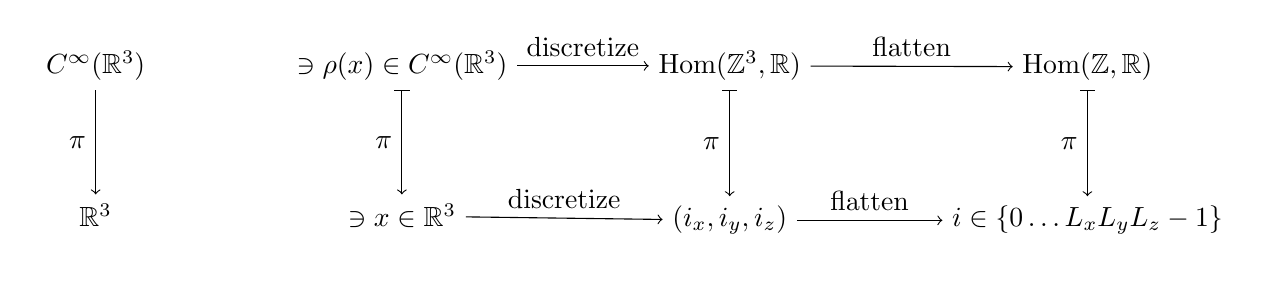
\begin{tikzpicture}
  \matrix (m) [matrix of math nodes, row sep=3.8em, column sep=4.8em, minimum width=2.9em] 
  {
   C^{\infty}(\mathbb{R}^3) & \ni \rho(x) \in C^{\infty}(\mathbb{R}^3) & \text{Hom}(\mathbb{Z}^3,\mathbb{R}) & \text{Hom}(\mathbb{Z},\mathbb{R}) \\
\mathbb{R}^3 & \ni x\in \mathbb{R}^3 & (i_x,i_y,i_z) & i \in \lbrace 0 \dots L_xL_yL_z - 1\rbrace \\
    };
  \path[->]
  (m-1-1) edge node [left] {$\pi$} (m-2-1)
  (m-1-2) edge node [above] {\text{discretize}} (m-1-3)
  (m-2-2) edge node [above] {\text{discretize}} (m-2-3)
  (m-1-3) edge node [above] {\text{flatten}} (m-1-4)
  (m-2-3) edge node [above] {\text{flatten}} (m-2-4)
  ;
  \path[|->]
  (m-1-2) edge node [left] {$\pi$} (m-2-2)
  (m-1-3) edge node [left] {$\pi$} (m-2-3)
  (m-1-4) edge node [left] {$\pi$} (m-2-4)
  ;
\end{tikzpicture} 
\]
Note that we can say that the discretization of $\rho(\mathbb{R}^3) \in C^{\infty}(\mathbb{R}^3)$ is a homomorphism $\text{Hom}$ from $\mathbb{Z}^3$ to $\mathbb{R}$ because vector space structure is preserved (and so discretization (discretize) is a functor, along with flatten).  As $C^{\infty}(N)$ is a vector space (ring) over the field $\mathbb{R}$ in that it is equipped with commutative (abelian) addition and scalar multiplication by field $\mathbb{R}$
\[
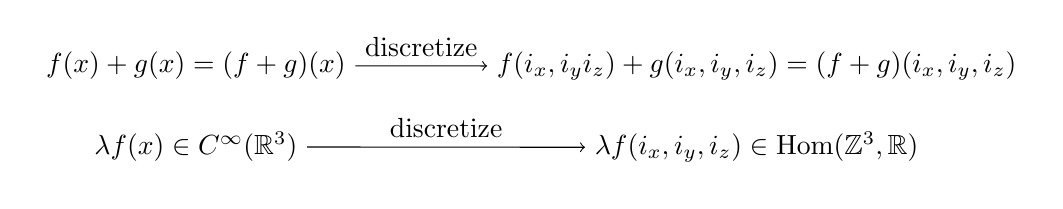
\begin{tikzpicture}
  \matrix (m) [matrix of math nodes, row sep=1.2em, column sep=4.8em, minimum width=2.9em] 
  {
    f(x) + g(x) = (f+g)(x) & f(i_x,i_yi_z) + g(i_x,i_y,i_z) = (f+g)(i_x,i_y,i_z) \\
    \lambda f(x) \in C^{\infty}(\mathbb{R}^3) &  \lambda f(i_x,i_y,i_z) \in \text{Hom}(\mathbb{Z}^3 , \mathbb{R}) \\
  };
  \path[->]
    (m-1-1) edge node [above] {\text{discretize}} (m-1-2)
  (m-2-1) edge node [above] {\text{discretize}} (m-2-2)
  ;
  \end{tikzpicture}
\]
Now consider the other object we need to consider, the vector bundle, namely the tangent bundle $TN$ over spatial (smooth) manifold $N$.  Namely consider the \emph{vector field}, representing the \emph{velocity vector field} $u$ as a section of the tangent bundle $T\mathbb{R}^3$ over Euclidean space (as a smooth manifold) $\mathbb{R}^3$.  Since $\text{dim}\mathbb{R}^3=3$, then the vector space $V \equiv T_xN$ ``over a fiber'' is of dimension 3, i.e. $\text{dim}T_xN$, $\forall \, x \in N$.
\[
u \in \mathfrak{X}(\mathbb{R}^3) = \Gamma(T\mathbb{R}^3)
\]
Recall the structure of a vector bundle, defined with a local trivialization $\varphi$ on an open set $U \subset N$:


\[
\begin{tikzpicture}
  \matrix (m) [matrix of math nodes, row sep=3.2em, column sep=4.8em, minimum width=2.9em] 
  {
TN \\
N \\
  };
  \path[->]
    (m-1-1) edge node [left] {$\pi$} (m-2-1)
  ;
  \end{tikzpicture} \qquad \, 
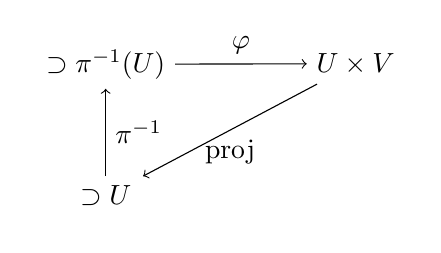
\begin{tikzpicture}
  \matrix (m) [matrix of math nodes, row sep=3.2em, column sep=4.8em, minimum width=2.9em] 
  {
\supset \pi^{-1}(U) & U\times V \\ 
\supset U & \\
  };
  \path[->]
    (m-1-1) edge node [above] {$\varphi$} (m-1-2)
  (m-2-1) edge node [right] {$\pi^{-1}$} (m-1-1)
  (m-1-2) edge node [below] {\text{proj}} (m-2-1)
  ;
  \end{tikzpicture}
\]

{\small 
Then consider its behavior under discretization (discretize functor):
\[
\begin{gathered}
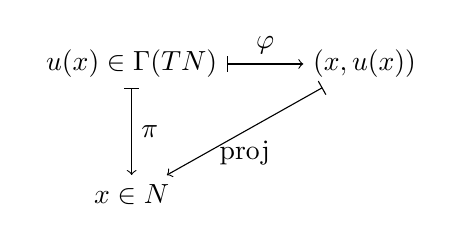
\begin{tikzpicture}
  \matrix (m) [matrix of math nodes, row sep=3.2em, column sep=2.8em, minimum width=2.4em] 
  {
u(x) \in \Gamma(TN) & (x,u(x)) \\ 
x\in N  & \\
  };
  \path[|->]
    (m-1-1) edge node [above] {$\varphi$} (m-1-2)
   edge node [right] {$\pi$} (m-2-1)
  (m-1-2) edge node [below] {\text{proj}} (m-2-1)
  ;
\end{tikzpicture} \xrightarrow{ \text{ discretize } } \\
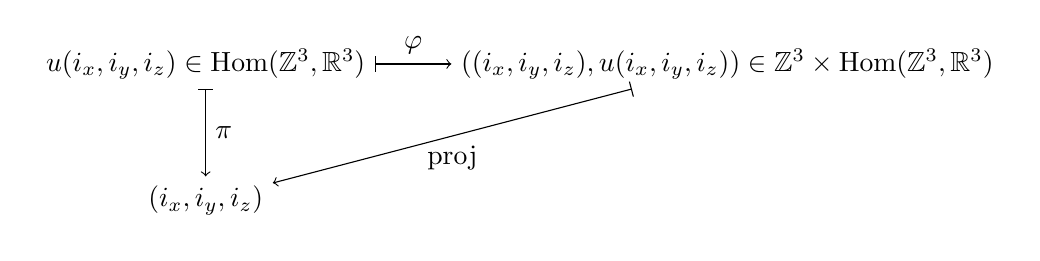
\begin{tikzpicture}
  \matrix (m) [matrix of math nodes, row sep=3.2em, column sep=2.8em, minimum width=2.4em] 
  {
u(i_x,i_y,i_z) \in \text{Hom}(\mathbb{Z}^3,\mathbb{R}^3) & ((i_x,i_y,i_z),u(i_x,i_y,i_z)) \in \mathbb{Z}^3 \times \text{Hom}(\mathbb{Z}^3 , \mathbb{R}^3) \\ 
(i_x,i_y,i_z)  & \\
  };
  \path[|->]
    (m-1-1) edge node [above] {$\varphi$} (m-1-2)
   edge node [right] {$\pi$} (m-2-1)
  (m-1-2) edge node [below] {\text{proj}} (m-2-1)
  ;
\end{tikzpicture}
\end{gathered}
\]
}

Nevertheless, the point is that the physical quantities we are concerned with, the scalar quantity of mass density $\rho$, or the velocity vector field $\mathbf{u}$, ``sit on top of'' spatial manifold $\mathbb{R}^3$.  They need to be transformed, for numerical computation, by some functor ``discretize'' so they sit on top of a grid $(\mathbb{Z}^+)^3$.  For CUDA C/C++, which on the device GPU only allows for 1-dimensional arrays that are on the contiguous global memory, there has to be a functor ``flatten'' that transforms those discretized versions of $\mathbb{R}^3$, $\rho$, $\mathbf{u}$ into what they'll be on the device GPU (note, at present, I am aware now that CUDA has its own 2-dimensional and 3-dimensional CUDA array, that is allocated on the device GPU in a different way than \verb|cudaMalloc|: I can explore the use of these specialized arrays in the future, hopefully with help from others).

One can think of $C^{\infty}(\mathbb{R}\times \mathbb{R}^3)$, time-dependent functions, such as $\rho = \rho(t\times \mathbf{x})$ and sections of the vector bundle, such as time-dependent velocity vector field $u(t,\mathbf{x}) \in \Gamma(\mathbb{R}\times \mathbb{R}^3)$ as \emph{objects} of a \emph{category}, the category of fiber bundles over $\mathbb{R}^3$.  If so, one can also expand on the idea expoused in Sage Math (cf. \href{http://doc.sagemath.org/pdf/en/reference/categories/categories.pdf}{Sage Reference Manual: Category Framework}), in that \emph{classes in C++ are categories in Category Theory} (i.e. math), \emph{objects in a class are objects in a category}, and \emph{class methods (or i.e. class functions) are functors in category theory}, so
\[
\begin{aligned}
  \text{ categories } & \longleftrightarrow  \text{ classes in C++ }  \\
  \text{ objects in a category } & \longleftrightarrow \text{ objects in a class } \\
  \text{ \text{Hom}s and functors } & \longleftrightarrow \text{ class methods or class functions }
\end{aligned}
\]

I will copy the one-line pitch that advocates for this software engineering framework from Sage Math (cf. \href{http://doc.sagemath.org/pdf/en/reference/categories/categories.pdf}{Sage Reference Manual: Category Framework}) here, replacing a few words for our case at present: \\

%\quote{
  One line pitch for mathematicians \\

\begin{quote} C++ and CUDA C++ classes provide a library of interrelated bookshelves, with each bookshelf containing algorithms,  tests, documentation, or some mathematical facts about the objects of a given category (e.g. groups, manifolds, vector bundles). \end{quote} 

%\quote{
One line pitch for programmers  \\

\begin{quote} Categories in Category Theory provide a large hierarchy of abstract classes for mathematical objects. To keep it maintainable, the inheritance information between the classes is not hardcoded but instead reconstructed dynamically from duplication free semantic information. \end{quote} 

So physical quantities $\rho$, $\mathbf{u}$, and energy per unit volume $\epsilon$ and momentum flux $\mathbf{p}$, that sit on $\mathbb{R}^3$ and are time-dependent, are implemented as objects in C++ classes.  There needs to be a different class for the CPU (``host'') and the GPU (``device'').  They are implemented in the folder \verb|physlib/| as \verb|R3grid.cpp|, \verb|R3grid.h| and \verb|dev_R3grid.cu|, \verb|dev_R3grid.h| for the host and device, respectively.  

\section{Heat equation}

Consider temperature $T$ and the temperature, in units of energy (joules, ergs, etc.), multiplied by the Boltzmann constant $k_B$, used as a units conversion factor, $\tau := k_BT$.

From Fick's law,
\[
\mathbf{j}_E = -\kappa \text{grad} \tau
\]
for (internal) energy $E$ of a thermodynamic system (of interest).

By the continuity equation (enforced by continuity),
\[
\frac{ \partial \epsilon }{ \partial t} + \text{div}\mathbf{j}_E = \frac{ \partial \epsilon }{ \partial t} + \text{div}(-\kappa \text{grad}\tau ) = \sigma_E
\]
where $\epsilon$ is the (internal) energy per unit volume (say $\epsilon := E /V$ for volume $V$ of the thermodynamic system), $\sigma_E$ is a heat source (if any).

Suppose for the thermodynamic system we're considering, we can write $\epsilon$ as
\[
\epsilon = c_V \tau
\]
where $c_V$ is the heat capacity at constant volume.

Then
\[
\begin{gathered}
\frac{ \partial \tau }{ \partial t} - \frac{ \kappa}{c_V} \Delta \tau = \frac{ \sigma_E }{ c_V} 
\end{gathered}
\]
or
\[
\begin{gathered}
\frac{ \partial T }{ \partial t} - \frac{ \kappa}{c_V} \Delta T = \frac{ \sigma_E }{ c_V k_B} 
\end{gathered}
\]
is the usual form of the heat equation.

Since the Laplacian, on $\mathbb{R}^3$, in Euclidean coordinates, consists of double derivatives (I'll use Einstein's summation notation where repeated indices imply summation):
\[
\Delta T \equiv \frac{ \partial^2 T}{ \partial (x^i)^2 } = \frac{ \partial ^2 T}{ \partial x^2 } + \frac{ \partial ^2 T}{ \partial y^2 } + \frac{ \partial ^2 T}{ \partial z^2 }
\]
finite difference methods can be used to numerically compute the heat equation.  Indeed, locally, away from external sources, the heat equation is
\[
\begin{gathered}
\frac{ \partial T }{ \partial t} =  \frac{ \kappa}{c_V} \Delta T   
\end{gathered}
\]

\section{Shared Memory on the GPU}

\subsection{Note on Memory model (in CUDA C/C++) of the device GPU}

In CUDA C/C++, for parallel programming or GPGPU on the device GPU, multiple number of threads $i$ are launched to do computations in parallel, asynchronously.  These threads can be arranged to be launched in blocks, so that the $j$th block can contain one or more threads that'll run a \emph{kernel} function (that does computation).

CUDA C/C++ (by default) gives you a way to reference or index a thread $i$, a block $j$ in a 2-dimensional, or up to a 3-dimensional ``model'' of the device memory.

Suppose \\
$L_i \equiv $ total number of threads to compute in the $i$th direction, $i=x,y,z$.  As we are discussing before about a grid $(L_x,L_y,L_z)$ that represents a subset of $\mathbb{R}^3$ where physics takes place, each grid point $(k_x,k_y,k_z) \in (L_x,L_y,L_z)$ is where computation occurs.  So $\forall \, (k_x,k_y,k_z)$ a thread will be launched.

A typical value of $(L_x,L_y,L_z)$ would be $640\times 640 \times 288$ for a grid of that size.

Let $M_i \equiv $ the total number of threads in a single block in the $i$th direction, $i=x,y,z$.

As $L_i$ and $M_i$ are positive integers, by integer arithmetic, in order to ensure all the threads we'd want to compute gets computed, the total number of blocks to be launched is given by the formula
\[
\frac{ L_i + M_i - 1}{ M_i}
\]
(I've worked it out in the \href{https://github.com/ernestyalumni/CompPhys/blob/master/LaTeXandpdfs/CompPhys.pdf}{CompPhys.pdf} writeup).

Suppose $i_x \in \lbrace 0 , \dots , M_x - 1\rbrace$ is the $i$th thread in block $(j_x,j_y,j_z) \in (N_x,N_y,N_z)$.  This corresponds to, in CUDA C/C++ code, \verb|threadIdx.x| for $(\verb|blockIdx.x|, \verb|blockIdx.y|, \verb|blockIdx.z| ) \in ( \verb|blockDim.x|, \verb|blockDim.y|, \verb|blockDim.z|)$.  \emph{Keep in mind this dictionary} between the math notation and CUDA C/C++ code.

Thus, the computation of the blocks needed, in the notation as mentioned above is as follows
\[
\begin{gathered}
  (L_x, L_y,L_z) \times (M_x,M_y,M_z) \xrightarrow{ \frac{ L_i + M_i - 1}{ M_i} = N_i } (N_x,N_y,N_z)
  \end{gathered}
\]
To obtain the thread's index along the $i$th direction, $i=x,y,z$, $k_i$, on the global memory of the device GPU, one needs to multiply the block index, $j_i$ (which would be \verb|blockIdx.x| or \verb|blockIdx.*| in general) by the block dimension in that direction, $M_i$ (which would be \verb|blockDim.x| or \verb|blockDim.*| in general).  This process is known as multiplying by the so-called ``stride'':
\[
k_i = i_i + j_i M_i = \lbrace 0 , \dots , N_i M_i - 1 \rbrace \qquad \, i = x,y,z
\]

As mentioned before, excepting that we're not allocating specialized CUDA 2 or 3 dimensional arrays on the device yet, we need a ``flatten'' functor, which would translate into a C++ class method, to obtain the thread's index on a 1-dimensional array.  This is done with this formula
\[
k := k_x + k_y L_x + k_z L_x L_y \in \lbrace 0 , \dots , L_x L_y L_z - 1 \rbrace
\]
As a note, we see here another opportunity to use constant memory in CUDA C/C++ by storing $L_x,L_y,L_z$ values in the constant memory, as each thread block will have to compute out $k$ each time a kernel function is run that requires $k$.  This also does double duty in representing the physical size (physics) of the system of interest, which is the grid size $(L_x,L_y,L_z)$.

\subsection{Shared memory via the so-called ``tiling'' scheme}

In calculating the heat equation, the so-called ``tiling'' scheme for using shared memory worked well.

The tile's dimension, $S_i$ is given by
\[
S_i := M_i  +2r  \qquad \, i = x,y,z
\]
where $r \equiv $ radius of the stencil or so-called ``halo'' cells.  

$r$ is exactly equal to the size of the stencil required for the desired (central) finite difference operator.  For instance, if a stencil of size 1 is required, i.e. coefficients $C_1$, values for $f$ at $f(x + 1*h)$, $f(x-1*h)$ is needed, then $r=1$ in $S_i$.  If a stencil of size 2 is required, i.e. coefficients $C_1, C_2$, and values for $f$ at $f(x+h), f(x-h), f(x+2h), f(x-2h)$, then $r=2$ in $S_i$ and so on.

In this tile of dimension $(S_x,S_y,S_z)$, the index $s_i$ in the $i$th direction, $i=x,y,z$, is given by the formula
\[
s_i := i_i + r\in \lbrace r, \dots M_i + r-1\rbrace
\]
Likewise, the ``striding'' that's needed to obtain the ``flattened'' thread index, $s_k$, in the tile is given by
\[
s_k := s_x + s_y S_x + s_z S_x S_y 
\]
where the $k$ subscript indicates that there is a 1-to-1 correspondence (bijection) between $s_k$ index on the tile to the $k$ index of the 1-dimensional array on the global memory.  

Note that in defining $s_i$ as such, we ensure, in the tile, that we have all the values needed to calculate the desired stencil of radius size $r$ at the thread $s_k \leftrightarrow k$.  

Then, the values of the array that lives on the global memory of the device GPU is loaded into shared memory of the tile size for each thread block, and this array in the shared memory is ``shared'' within threads of the (single) thread block.  

This is implemented in 2-dimensions and 3-dimensions for the heat equation in \verb|heat2d| and \verb|heat3d|.  

\section{Euler equations (Navier-Stokes equation for inviscid (i.e. nonviscous) flow) in 2 and 3 dimensions with finite difference}

Armed with the divergence and gradient $\text{div}$, $\text{grad}$, we can attempt to numerically compute the Euler equations on the largest possible grid allowed by the device GPU's global memory (6 GB on the NVIDIA GeForce GTX 980Ti that I have; in practice, less than 6 GB is available since I'd need some for video display and the OpenGL graphics rendering).  Along this line, as we need the mass density $\rho \in C^{\infty}(\mathbb{R}^3)$, (bulk) fluid velocity vector field $\mathbf{u} \in \mathfrak{X}(\mathbb{R}^3)$, momentum density $\mathbf{p} := \rho \mathbf{u} \in \mathfrak{X}(\mathbb{R}^3)$, and total energy per unit volume $\epsilon \in C^{\infty}(\mathbb{R}^3)$ to be represented by flattened arrays of floats, \verb|float3|'s, \verb|float3|'s, and floats, respectively, each of size 8, 24, 24, and 8 bytes, respectively, theoretically, on my GTX 980Ti, a 3-dimensional grid of size $900\times 900 \times 900$ can be implemented.  In practice, because of the device's limitations on the total number of blocks that can be launched and the total number of threads that can be launched in the $z$ direction, and trying to obtain computations that can be done in real-time, I launched grids of size $640 \times 640 \times 288$, which still is about 118 million grid points, only about 1/6 the total number of grid points theoretically possible.

My interest in the Euler equations is in modeling (compressible) gas dynamics between the combustion chamber and out to the nozzle of a liquid-propellant rocket engine.  For high enough Reynolds number $\text{Re}$, the viscosity of the gas is neglected and hence the adjective ``inviscid'' of inviscid flow.

The Euler equations are the following, in its differential form (valid for a fixed volume $V$ that's small enough):
\begin{equation}
\begin{gathered}
  \frac{ \partial \rho }{ \partial t} + \text{ div}( \rho \mathbf{u} ) = 0 \\ 
  \frac{ \partial p^i }{ \partial t} + \text{ div}( p^i \mathbf{u} ) = - (\text{grad}p)^i \qquad \, \forall \, i = x,y,z \\
  \frac{ \partial \epsilon}{ \partial t} + \text{div}( h \mathbf{u} ) = 0
  \end{gathered}
  \end{equation}
where $\mathbf{p} := \rho \mathbf{u}$ is the momentum density, with components $p^i$, \, $\forall \, i = x,y,z$, $p$ is the pressure, and $\epsilon$ is the total energy per unit volume, $h$ is the total enthalpy per unit volume (which should be remarked of which it also includes the kinetic energy per unit volume $k:= \frac{1}{2} \rho u^2$, i.e. $h := h' + k$).

For the ideal or perfect gas, given us the so-called ``equation of state'', pressure $p$ is given by
\[
p = (\gamma - 1) (\epsilon - \frac{1}{2} \rho u^2)
\]
and so the second equation, that describes momentum dynamics (i.e. $F=ma$), can be written entirely in terms of $\rho, \mathbf{p}, \mathbf{u}$, and $\epsilon$.

Also from this equation of state, the third equation of the Euler equations, governing energy conservation, can be written as
\[
\frac{ \partial \epsilon }{ \partial t} = -\text{div}(\gamma \epsilon \mathbf{u}) - \text{div}(k\mathbf{u}(1-\gamma ) )
\]
where $\gamma$ is the usual heat capacity ratio.  

Note that in writing Euler's equations above, I followed Le Bellac, Mortessagne, Batrouni (2004) \cite{MLeBellacFMortessagneGBatrouni2004}.  One should note that $\epsilon$ is the total energy per unit volume, and not the total energy per unit mass.  The reasons for this are the following.  Le Bellac, Mortessagne, Batrouni (2004) \cite{MLeBellacFMortessagneGBatrouni2004} carefully derives convection of a thermodynamic system down to the insertion of a \emph{single} molecule into a thermodynamic system, and how it has to change the entropy of the thermodynamic system.  I have also recapped and added details to clarify this derivation in my notes in \href{https://github.com/ernestyalumni/Propulsion/blob/master/LaTeXandpdfs/Propulsion.pdf}{Propulsion.pdf}.  The difference between the so-called ``stagnation'' enthalpy and the ``stagnation'' (internal) energy (for the thermodynamic system) and the enthalpy and (internal) energy that includes the kinetic energy is clarified in this derivation.  In fact, they are related by changes in reference frames, Galilean transformations or Galilean ``boosts''.  However, what must hold true, what must be an agreed-upon physical principle, is that the entropy is a Galilean invariant; entropy cannot change under changes of reference frames (otherwise the second thermodynamic law is violated).

So this derivation is true down to the insertion of a single molecule into a fixed volume $V$.  This is important because prior to the insertion, the mass density of the gas of interest in this fixed volume $V$ is $0$.  Euler's equations written as such above avoids division by $0$ via division by $\rho$.  The energy of inside a fixed volume $V$ with no gas in it should be $0$.  So $\epsilon =0$.  However, if we were considering the energy per unit mass, it would be undefined.

This is also important in numerical computation as it avoids division by zero errors.

This is implemented in 2-dimensions in \verb|Euler2d/physlib| in \verb|convect.cu| and \verb|convect.h|.  Shared memory is utilized, but not the ``tiling'' scheme; it's used for the stencil values needed for finite difference.

As before, this code can be easily implemented for 3-dimensions.  

\section{Miscellaneous Notes}

\subsection{C++11/C++14}

I used the \verb|functional| library to interact well with OpenGL, inherently a C API.  With \verb|nvcc| as of right now, CUDA Toolkit 7.5, you cannot factor code into C++ classes that'll compile with \verb|nvcc| compiler.  But you can use \verb|functional| to make functionals that'll output out functions for OpenGL.  


\begin{thebibliography}{9}
\bibitem{MLeBellacFMortessagneGBatrouni2004}
Michel Le Bellac, Fabrice Mortessagne, G. George Batrouni.  \textbf{Equilibrium and Non-Equilibrium Statistical Thermodynamics}.  Cambridge University Press (May 3, 2004).  ISBN-13: 978-0521821438

\end{thebibliography}

\end{document}
